\documentclass[crop,tikz]{standalone}
\usepackage{pgfplots}

\usetikzlibrary{arrows.meta}

% Vector field of a homogeneously electrically charged and rotating
% sphere of Radius R. In spherical coordinates, the magnetic field is
%
% \vec{B}(r,\theta,\varphi)
%   = \mu_0 m/(4\pi r^3)[3\vec{e}_r(\vec{e}_z\cdot\vec{e}_r) - \vec{e}_z]
%   = \mu_0 m/(4\pi r^3)[2\cos(\theta)\vec{e}_r + \sin(\theta)\vec{e}_\theta],
%
% where m = q\omega R^2/3 is the magnetic moment, q is the total
% charge of the sphere, \omega is the angular frequency of the
% rotation and \theta\in[0;\pi] and \varphi\in[0;2\pi).

\pgfplotsset{
  compat=1.18,
  inverted/.style = {
    every axis legend/.append style={
      draw=white,
      fill=hardblack,
      text=white
    }
  },
}

\usetikzlibrary{decorations.markings,arrows.meta}

\tikzset{
  fieldline/.style={
    red,
    thin,
    postaction={decorate},
    decoration={
      markings,
      mark=at position 0.5 with {\arrow{Latex[length=1mm]}}
    }
  },
}

\begin{document}
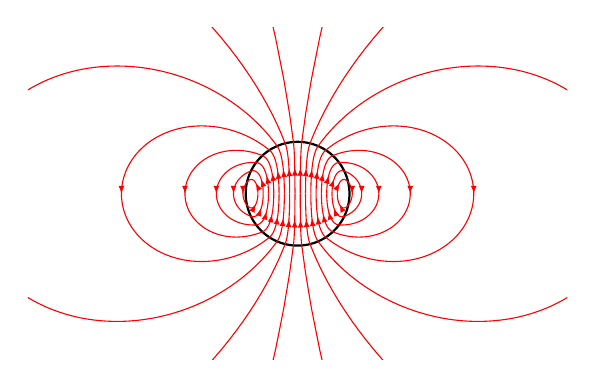
\begin{tikzpicture}
  \begin{axis}[
    hide axis,
    axis equal image,
    xlabel={$x$},
    ylabel={$z$},
    xmin=-5.2, xmax=5.2,
    ymin=-3.2, ymax=3.2,
    samples=150,
    % clip=false,
    ]
    % radius of sphere
    \pgfmathsetmacro{\R}{1}
    % sphere
    \addplot[black, thick, domain=0:360] ({\R*cos(x)}, {\R*sin(x)});
    % maximum x value inside sphere
    \pgfmathsetmacro{\xmaxPhys}{sqrt(2/3)*\R}
    % number of field lines
    \pgfmathsetmacro{\Nlines}{8}
    % loop over number of field lines
    \pgfplotsinvokeforeach{0,1,2,3,4,5,6,7}{
      % equidistant x-coordinate on positive x-axis
      \pgfmathsetmacro{\xzero}{(#1+0.5)*\xmaxPhys/\Nlines}
      % u_0 = x_0^2/R^2
      \pgfmathsetmacro{\uzero}{(\xzero/\R)^2}
      % K = u_0(5 - 3u_0)
      \pgfmathsetmacro{\K}{\uzero*(5-3*\uzero)}
      % corresponding outer fieldline parameter c
      % r = c sin^2(theta)
      \pgfmathsetmacro{\cVal}{2*\R/\K}
      % -------------------------
      % outside sphere
      % r = c sin^2(theta)
      % -------------------------
      \pgfmathsetmacro{\thetamin}{asin(sqrt(\R/\cVal))}
      \pgfmathsetmacro{\thetamax}{180-\thetamin}
      % right outer fieldline
      \addplot[
        fieldline,
        domain={\thetamin}:{\thetamax},
      ] ({\cVal*sin(x)^3}, {\cVal*sin(x)^2*cos(x)});
      % left outer fieldline
      \addplot[
        fieldline,
        domain={\thetamin}:{\thetamax},
      ] ({-\cVal*sin(x)^3}, {\cVal*sin(x)^2*cos(x)});
      % -------------------------
      % inside sphere
      % u(5-3u) sin^2(theta) = K
      % -------------------------
      % upper right inner fieldline
      \addplot[
        fieldline,
        domain={\uzero}:1,
      ] ({\R*sqrt(\K/(5-3*x))}, {\R*sqrt(x)*sqrt(max(0,1-\K/(x*(5-3*x))))});
      % lower right inner fieldline
      \addplot[
        fieldline,
        domain=1:{\uzero},
      ] ({\R*sqrt(\K/(5-3*x))}, {-\R*sqrt(x)*sqrt(max(0,1-\K/(x*(5-3*x))))});
      % upper left inner fieldline
      \addplot[
        fieldline,
        domain={\uzero}:1,
      ] ({-\R*sqrt(\K/(5-3*x))}, {\R*sqrt(x)*sqrt(max(0,1-\K/(x*(5-3*x))))});
      % lower left inner fieldline
      \addplot[
        fieldline,
        domain=1:{\uzero},
      ] ({-\R*sqrt(\K/(5-3*x))}, {-\R*sqrt(x)*sqrt(max(0,1-\K/(x*(5-3*x))))});
    }
  \end{axis}
\end{tikzpicture}
\end{document}
